\documentclass[11pt]{article}
\usepackage[margin=1in]{geometry} 
\usepackage{amsmath}
\usepackage{tcolorbox}
\usepackage{amssymb}
\usepackage{amsthm}
\usepackage{commath}
\usepackage{lastpage}
\usepackage{fancyhdr}
\usepackage{accents}
\usepackage{csquotes}
\usepackage{soul}
\newcommand{\ubar}[1]{\underaccent{\bar}{#1}}
\pagestyle{fancy}
\setlength{\headheight}{40pt}


\newenvironment{solution}
  {\renewcommand\qedsymbol{$\blacksquare$}
  \begin{proof}[Solution]}
  {\end{proof}}
\renewcommand\qedsymbol{$\blacksquare$} 
\begin{document}

\lhead{Yida Liu} 
\rhead{EECS 416 Spring 2020 \\ Convex Optimization for Engineering \\ Homework 3} 
\cfoot{\thepage\ of \pageref{LastPage}}

\section{Classify Breast Cancer with SVM}
\subsection{Train SVM}
First, we define a set of variables
\begin{enumerate}
    \item $a$: the hyperplane coefficients
    \item $b$: the hyperplane bias
    \item $u_x$ and $v_y$: "slack" variables
    \item $\tau$: penalty parameter
    \item $M$ and $B$: the malicious and benign observations
\end{enumerate}
Based on these variables, we formulate our Support Vector Machine as follows: 
\begin{align*}
&\min&& \frac{1}{2}\|a\| + \tau(\sum_{x\in M} u_x + \sum_{y \in B} v_y)\\
&s.t.&& -xa + b - u_x \leq -1 & \forall x \in M \\
&&& ya - b - v_y \leq -1 & \forall y \in B \\
&&& u_x, v_y \geq 0 &\forall x \in M, y \in B\\
\end{align*}

We construct and solve for the hyperplane using MATLAB \texttt{quadprog}. The result is presented in Table \ref{tab:svm_param}.

We examine the slack variables to determine whether the data is separable. When the slack variable for an observation is 0, it means that the observation can be classified into one of the classes without ambiguity, otherwise it is an outlier. We examined all 500 observations and found that 488 of them has a binding slack variable. That is, there are only 12 outliers. Therefore, the data is actually, for the most part, separable. 



\subsection{Test SVM}
Table \ref{tab:svm_test} displays test result of the hyperplane found by quadprog.

\begin{table}[h]
    \centering
    \begin{tabular}{c || c | c}
         metric & Malicious & Benign  \\
         \hline
         number of people & 17 & 69 \\
         \hline
         accuracy & 100\% & 94.23\% \\ 
         sensitivity and specitivity & 0\% & 1.92\% \\
         unclassified & 0 & 3.85\%\\
    \end{tabular}
    \caption{Result for Testing the SVM Hyperplane Classification}
    \label{tab:svm_test}
\end{table}

\begin{table}
    \centering
    \begin{tabular}{c c}
 a & b\\
 \hline
 \hline
   -7.0337 & 25.8190\\
   -0.0094\\
    0.6434\\
    0.0328\\
    2.4662\\
  -14.3500\\
   -6.4099\\
   11.4022\\
    7.6009\\
    2.3617\\
    0.5795\\
   -1.7769\\
   -0.6713\\
    0.1779\\
    8.6950\\
  -18.6120\\
  -21.9553\\
    8.9804\\
   -6.2920\\
   -3.2782\\
    1.9325\\
    0.3383\\
    0.0910\\
   -0.0209\\
   31.8356\\
  -12.1760\\
   12.4716\\
   24.7374\\
   12.0669\\
    8.2213\\
    \end{tabular}
    \caption{SVM Hyperplane Parameters for Problem 1}
    \label{tab:svm_param}
\end{table}

\section{Portfolio Investment}

We solve for the model 
\begin{align*}
&\max&& r^Tx - \alpha x^TVx\\
&s.t.&& \sum x_i = 1 \\
&&& x_i \geq 0, \forall x
\end{align*}

We use MATLAB to solve for the optimal portfolio given alpha. Table \ref{tab:hw3_p2_portfolio} presents the chosen alpha, 3 most invested stock, mean and variance. Figure \ref{fig:hw3_prob2_eff} shows the efficient frontier under the model with the rate of return and variance when investing each of the 30 stocks only.

\begin{table}[]
    \centering
    \begin{tabular}{ccccccccc}
$\alpha$  & stock 1 & ratio 1 &  stock 2 & ratio 2 &  stock 3 & ratio 3 & $\mu$ & $\Sigma$ \\
\hline \hline
1 & 5 & 1 & 8 & \text{8.6673e-16} & 28 & \text{2.6180e-17} & 0.0132 & 0.0011\\
2 & 5 & 1.000 & 8 & \text{1.7368e-07} & 28 & \text{7.7011e-09} & 0.0132 & 0.0011\\
5 & 5 & 0.5570 & 8 & 0.3234 & 28 & 0.1196 & 0.0120 & \text{7.9121e-04}\\
10 & 28 & 0.3123 & 18 & 0.2653 & 8 & 0.1643 & 0.0086 & \text{3.0863e-04}\\
20 & 18 & 0.5037 & 28 & 0.3134 & 14 & 0.1760 & 0.0070 & \text{1.7867e-04}\\
50 & 18 & 0.3500 & 28 & 0.2254 & 17 & 0.1701 & 0.0058 & \text{1.4088e-04}\\
80 & 18 & 0.2770 & 28 & 0.2075 & 17 & 0.1803 & 0.0050 & \text{1.2897e-04}\\
100 & 18 & 0.2450 & 28 & 0.1961 & 24 & 0.1818 & 0.0047 & \text{1.2527e-04}    \end{tabular}
    \caption{Optimal Portfolio with 3 Most-Invested Stocks for Selected Values of $\alpha$}
    \label{tab:hw3_p2_portfolio}
\end{table}


\begin{figure}
    \centering
    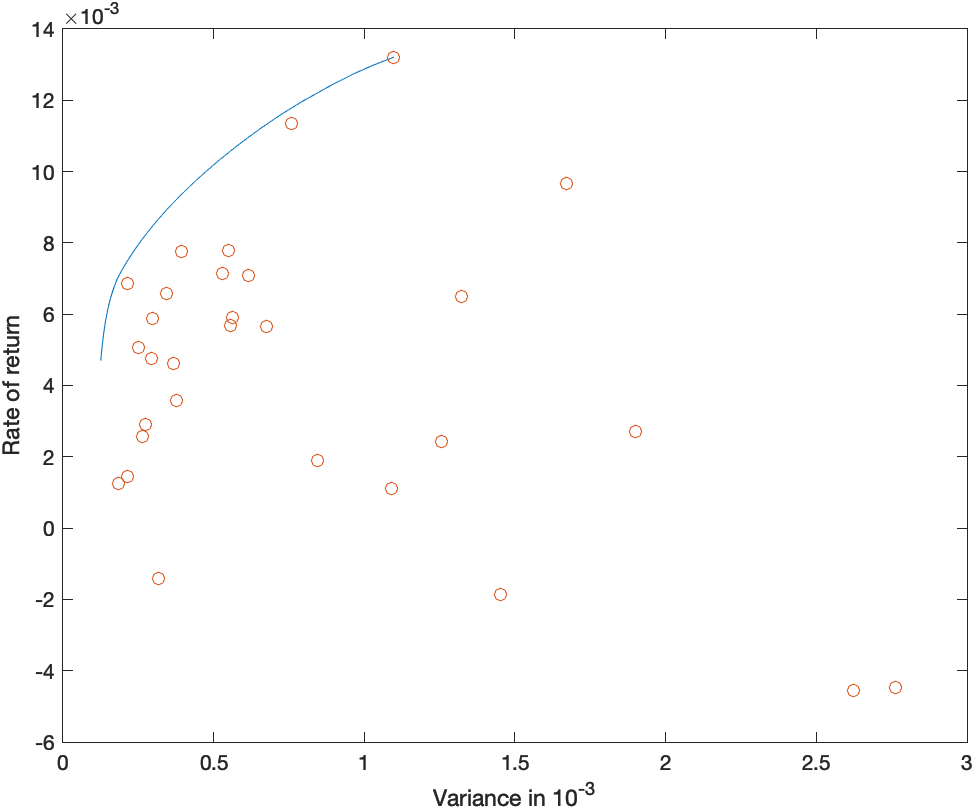
\includegraphics[width=0.5\linewidth]{hw3/prob2_plot.png}
    \caption{Efficient Frontier with Each Individual Stock Investment Marked}
    \label{fig:hw3_prob2_eff}
\end{figure}

\section{Feasible Region}
\begin{enumerate}
    \item $(0.5, 0.5)$ is a feasible point inside the boundary.
    \item $(1, 0)$ is a feasible point on the boundary.
    \item $(-1, 0)$ is a feasible point on the boundary.
    \item $(\frac{1}{\sqrt{2}},\frac{1}{\sqrt{2}})$ is a feasible point on the boundary.
\end{enumerate}
Figure \ref{fig:hw3_p3_feasible} shows the feasible region enclosed by the boundary set $\mathbf{X}$.
\begin{figure}
    \centering
    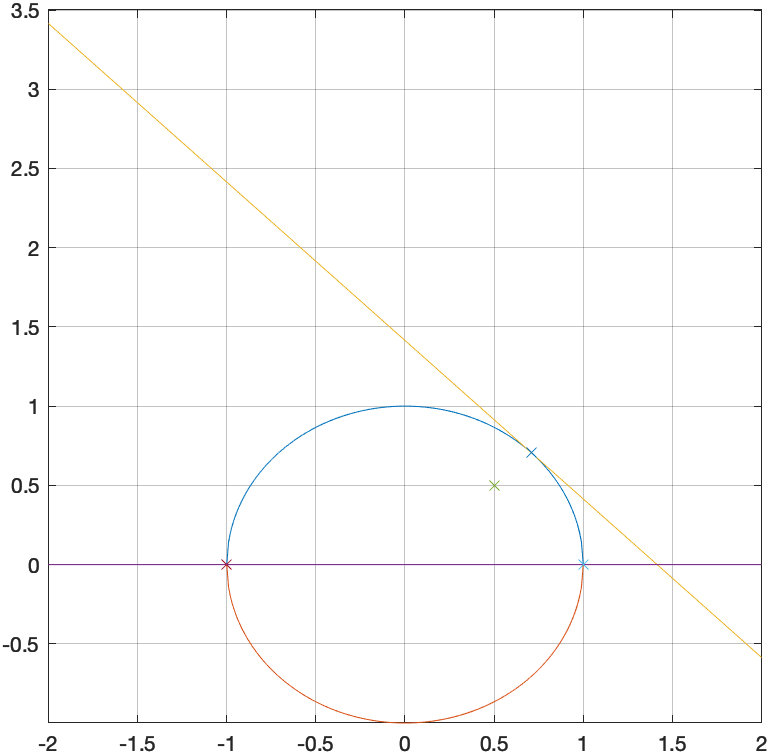
\includegraphics[width=0.5\linewidth]{hw3/prob3_plot.png}
    \caption{Feasible Region Enclosed by $\mathbf{X}$}
    \label{fig:hw3_p3_feasible}
\end{figure}


\begin{figure}
    \centering
    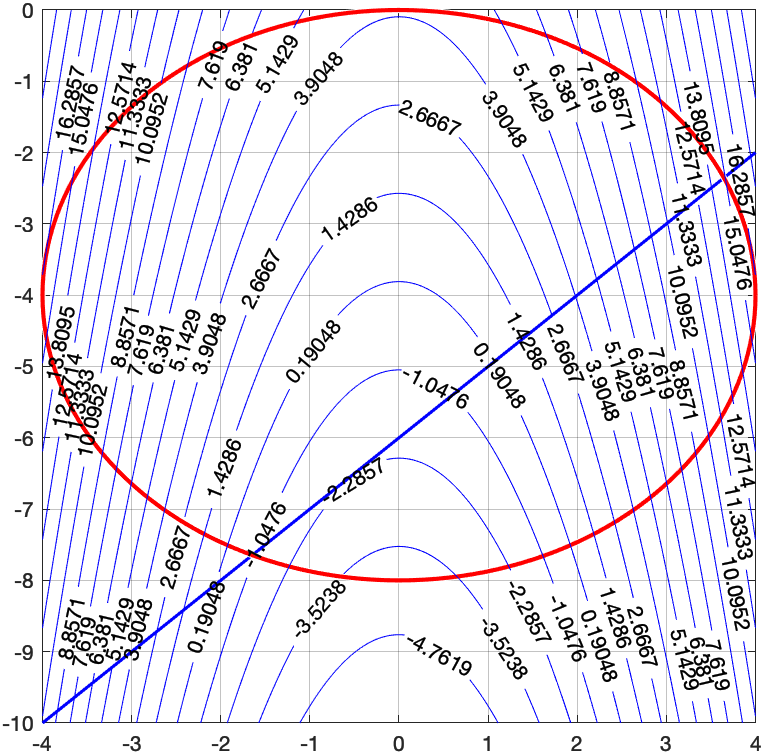
\includegraphics[width=0.5\linewidth]{hw3/prob4_plot.png}
    \caption{Contour Plot with Constraints by Graphical Method}
    \label{fig:hw3_prob4_contour}
\end{figure}

\section{Solve with Graphical Method}
We show a contour plot with feasible region enclosed by the constraint in Figure \ref{fig:hw3_prob4_contour}.
\begin{enumerate}
\item The optimal solution happens at $(0, -8)$, which gives an objective value of -4.
\item The feasible region is the intersection between region below line (in blue) and the circle (in red). 
\item There are local minimum and maximum within the bounded region. However, the function itself grows without bound (toward +/- infinity). 



\end{enumerate}

\begin{figure}
    \centering
    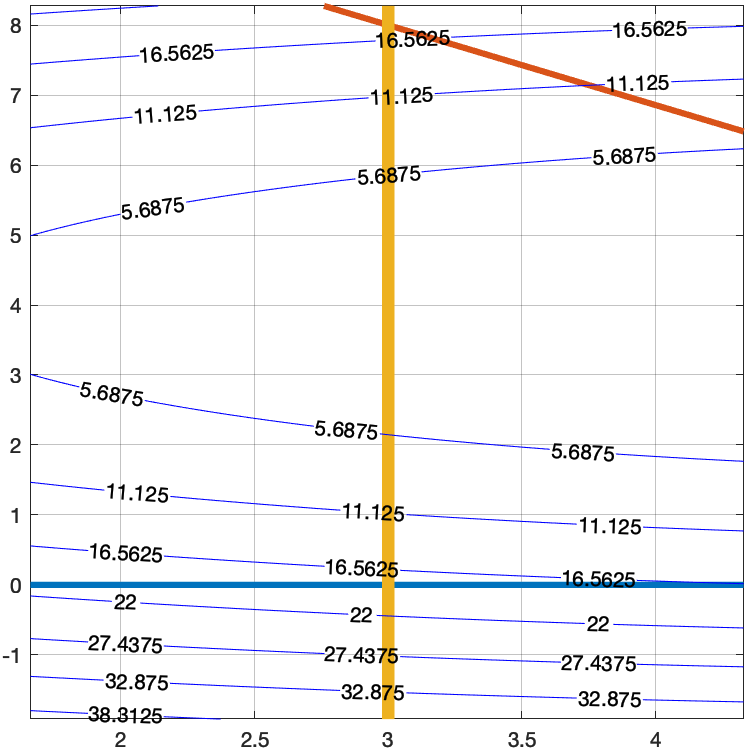
\includegraphics[width=0.5\linewidth]{hw3/prob5_plot.png}
    \caption{Contour Plot by Graphical Method 2}
    \label{fig:hw3_prob5_contour}
\end{figure}
\section{Solve with Graphical Method 2}

We show a contour plot with feasible region enclosed by the constraints in Figure \ref{fig:hw3_prob5_contour}.

\begin{enumerate}
\item The optimal solution happens at $(3, 4)$, which gives an objective value of $\frac{9}{4}$.
\item The feasible region is the $x_1=3$ line (in yellow) segment lies between $x_2=\frac{80}{7} = \frac{8}{7}x_1$ (in red) and $x_2=0$ (in blue).
\item There are local minimum and maximum within the bounded region. There are also global minimum in the center point, and no global maximum as the function grows infinitely.
\end{enumerate}

\section{Minimizers and Constraint Substitution}

\subsection{Identify all local minimizer and maximizer}

\begin{figure}
    \centering
    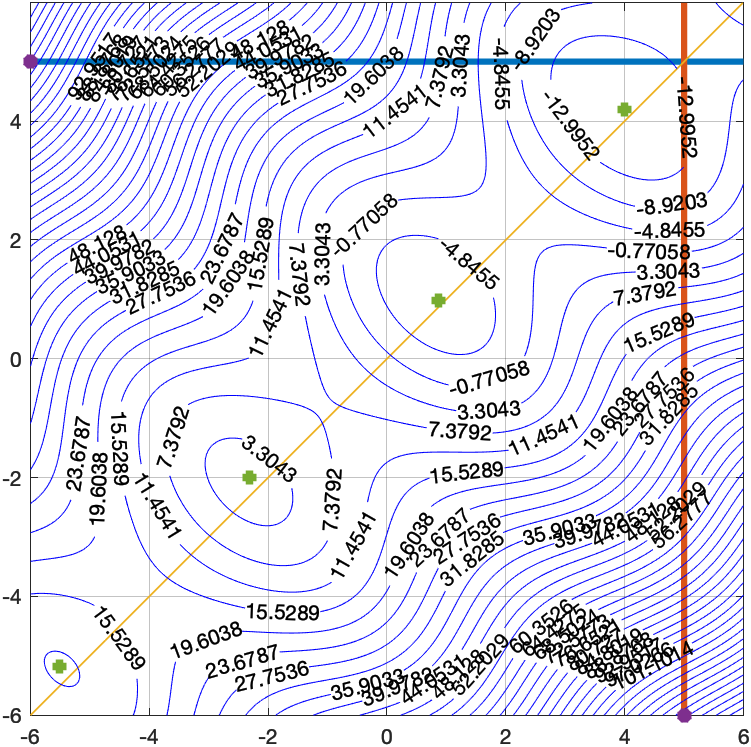
\includegraphics[width=0.5\linewidth]{hw3/prob6_plot.png}
    \caption{Contour Plot of Given Non-Linear Programming Problem}
    \label{fig:hw3_prob6_contour}
\end{figure}


We show a contour plot in Figure \ref{fig:hw3_prob6_contour}. The lines perpendicular to x-axis (in red) and y-axis (in blue), together, form the boundary of the feasible region. In addition, we also placed $y=x$ (in yellow) for identify points. We can see that along the $y=x$ (in yellow), there are a few local minimizer (marked in green); the funtion itself grows towards plus infinity toward the top-left and bottom-right direction, but within the bounded region, we have two local maximizer in $(-6, 5)$ and $(5, -6)$ (marked in purple).

\subsection{Convert to Unconstrained Problem}

\begin{align*}
&\min&& -5\sin(10-y_1^2 - y_2^2) + (y_2^2-y_1^2)^2+y_1^2+2y_2^2-15\\
&&& \text{unconstrained}
\end{align*}


\end{document}